 \documentclass[20pt]{beamer}
\usepackage[utf8]{inputenc}
\usepackage[utf8]{vietnam}
\usepackage{amsmath}
\usepackage{amsfonts}
\usepackage{amssymb}
\usepackage{graphicx}
\usepackage{xcolor}
\usepackage{utopia} %font utopia imported

\usepackage{ragged2e}
\usepackage{etoolbox}

\mode<beamer>{\usetheme{CambridgeUS}}

\usecolortheme{default}

\usepackage{hyperref}
\hypersetup{pdfpagemode=FullScreen} %mode FullScreen with beamer

\apptocmd{\frame}{}{\justifying}{} % Allow optional arguments after frame.

\usepackage{comment}

\makeatletter
\let\insertuniversity\relax
\newcommand\universitytitle{TRƯỜNG ĐH}

\let\insertclass\relax
\newcommand\classtitle{Lớp}

\let\insertcourse\relax
\newcommand\coursetitle{Môn học}

\mode<all>
{
  \newcommand\university[1]{\def\insertuniversity{#1}}
  
  \newcommand\class[1]{\def\insertclass{#1}}
  
  \newcommand\course[1]{\def\insertcourse{#1}}
  \titlegraphic{}
}

\defbeamertemplate*{title page}{supdefault}[1][]
{
  \begingroup
    \centering
    \ifx\insertuniversity\relax\relax\else
    \begin{beamercolorbox}[sep=2pt,center,#1]{author}
      \footnotesize\universitytitle~\insertuniversity
    \end{beamercolorbox}\fi
    
    \begin{beamercolorbox}[sep=8pt,center,#1]{title}
      \usebeamerfont{title}\Large\inserttitle\par%
      \ifx\insertsubtitle\@empty\relax%
      \else%
        \vskip0.25em%
        {\usebeamerfont{subtitle}\usebeamercolor[fg]{subtitle}\insertsubtitle\par}%
      \fi%     
    \end{beamercolorbox}%
    \vskip.5em\par

    \vspace{-.3cm}
    \ifx\insertcourse\relax\relax\else
    \begin{beamercolorbox}[sep=6pt,center,#1]{author}
      \usebeamerfont{author}\small\coursetitle:~\insertcourse
    \end{beamercolorbox}\fi
    %\vspace{-.3cm}
    \ifx\insertclass\relax\relax\else
    \begin{beamercolorbox}[sep=6pt,center,#1]{author}
      \usebeamerfont{author}\small\classtitle:~\insertclass
    \end{beamercolorbox}\fi

    %\vspace{-.3cm}
    \begin{beamercolorbox}[sep=6pt,center,#1]{author}
      \usebeamerfont{author}\small\insertauthor
    \end{beamercolorbox}
    %\begin{beamercolorbox}[sep=8pt,center,#1]{institute}
      %\usebeamerfont{institute}\insertinstitute
    %\end{beamercolorbox}
    %\vspace{-.3cm}
    \begin{beamercolorbox}[sep=8pt,center,#1]{date}
      \usebeamerfont{date}\small\insertdate
    \end{beamercolorbox}\vskip0.5em
    {\usebeamercolor[fg]{titlegraphic}\inserttitlegraphic\par}
  \endgroup
  \vfill
}
\setbeamertemplate{title page}[supdefault][colsep=-4bp,rounded=true,shadow=\beamer@themerounded@shadow]\makeatother

%Title page
\title[Van điện]{\emph{Chủ đề báo cáo}\\VAN ĐIỆN}
\author[Điều khiển quá trình]{GVHD: Nguyễn Ngô Phong \and SVTH: Nhóm 6}
\course{Điều khiển quá trình}
\class{Công nghệ, kỹ thuật điện, điện tử}
\university{KỸ THUẬT -- CÔNG NGHỆ CẦN THƠ}
\date[Nhóm 6]{\today}
%\date[Nhóm 1]{Ngày 24 tháng 08 năm 2016}

%\logo{\includegraphics[height=1.3cm]{logo_ctut.pdf}}

\AtBeginSection[]
{
  \begin{frame}
    \frametitle{Nội dung báo cáo}
    \justifying
    \tableofcontents[currentsection]
  \end{frame}
}
\definecolor{doden}{RGB}{204, 0, 0}
\begin{document}
%http://tex.stackexchange.com/questions/82794/removing-page-number-from-title-frame-without-changing-the-theme
\bgroup
\makeatletter
\setbeamertemplate{footline}
{
  \leavevmode%
  \hbox{%
  \begin{beamercolorbox}[wd=.333333\paperwidth,ht=2.25ex,dp=1ex,center]{author in head/foot}%
    \usebeamerfont{author in head/foot}\insertshortauthor\expandafter\beamer@ifempty\expandafter{\beamer@shortinstitute}{}{~~(\insertshortinstitute)}
  \end{beamercolorbox}%
  \begin{beamercolorbox}[wd=.333333\paperwidth,ht=2.25ex,dp=1ex,center]{title in head/foot}%
    \usebeamerfont{title in head/foot}\insertshorttitle
  \end{beamercolorbox}%
  \begin{beamercolorbox}[wd=.333333\paperwidth,ht=2.25ex,dp=1ex,right]{date in head/foot}%
    \usebeamerfont{date in head/foot}\insertshortdate{}\hspace*{2em}
%    \insertframenumber{} / \inserttotalframenumber\hspace*{2ex} 
    \hspace*{6ex}
  \end{beamercolorbox}}%
  \vskip0pt%
}

\begin{frame}
\titlepage
\end{frame}
\egroup

\setcounter{framenumber}{0}

%--------------------------------------------------------------------------------
%--------------------------------------------------------------------------------
% Danh sach thanh vien
\begin{frame}{Danh sách thành viên}
	\vspace{-1cm}
	\begin{small}
	\begin{columns}
		\column{0.6\textwidth}
		\begin{enumerate}
			\item Nguyễn Văn Bảy
			\item Nguyễn Văn Đình
			\item Thi Minh Nhựt
			\item Nguyễn Văn Quy
			\end{enumerate}

		\column{0.6\textwidth}
		\begin{enumerate}	% Danh sach tiep theo
			\setcounter{enumi}{4}
			\item Phạm Thanh Quý
			\item Hồ Minh Thành
			\item Liên Thái Trường
			\item Phan Thành Tuấn
		\end{enumerate}
	\end{columns}
	\end{small}
\end{frame}

%--------------------------------------------------------------------------------
%--------------------------------------------------------------------------------
% Noi dung bao cao
\begin{frame}	%Trang muc luc
	\frametitle{Nội dung báo cáo}
	\tableofcontents
\end{frame}

\section{Giới thiệu van điện}
\subsection*{Khái niệm}
\begin{frame}{Khái niệm}
\justifying
\alert{Van điện} có \textcolor{blue}{cơ chế chấp hành là động cơ bước hoặc động cơ servo}, được \textcolor{blue}{điều khiển trực tiếp bằng tín hiệu ra của của bộ điều khiển} (dòng từ $4-20mA$ hoặc tín hiệu số).
\end{frame}

\begin{frame}{Động cơ bước, động cơ servo}
\vspace{-.5cm}
\begin{center}
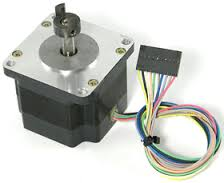
\includegraphics[scale=.8]{images/dong-co-buoc.jpg} 
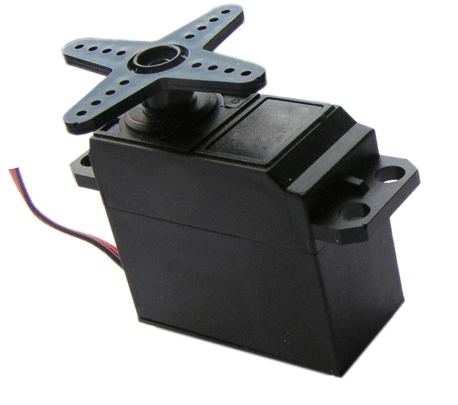
\includegraphics[scale=.35]{images/servo-motor.png} 
\end{center}
\end{frame}
\subsection*{Chức năng}
\begin{frame}{Chức năng}
\justifying
\alert{Van điện có thể làm được:} \textcolor{blue}{chuyển đổi trạng thái của van} hoặc \textcolor{blue}{mở van một góc nhất định}.

\alert{Phạm vi áp dụng:} dùng trong các ứng dụng nhỏ đòi hỏi \textcolor{blue}{độ chính xác cao}.
\end{frame}

\section{Cấu tạo và Nguyên lý của van điện}
\subsection*{Cấu tạo van điện}
\begin{frame}{Cấu tạo van điện}
\begin{itemize}
	\item Phần van cơ thông thường.
	\item Phần điều khiển bằng điện
\end{itemize}
\end{frame}

\begin{frame}{Cấu tạo van điện}
	\vspace{-.3cm}
	\begin{center}
		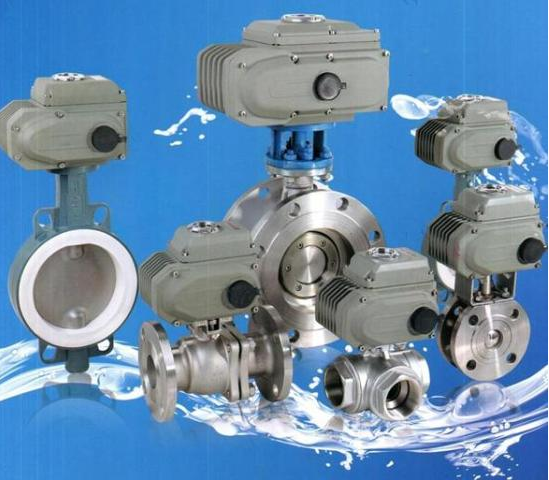
\includegraphics[scale=.4]{images/vi-du-van-dien.png} 
	\end{center}
\end{frame}

\begin{frame}{Cấu tạo van điện}
	\vspace{-.55cm}
	\begin{center}
		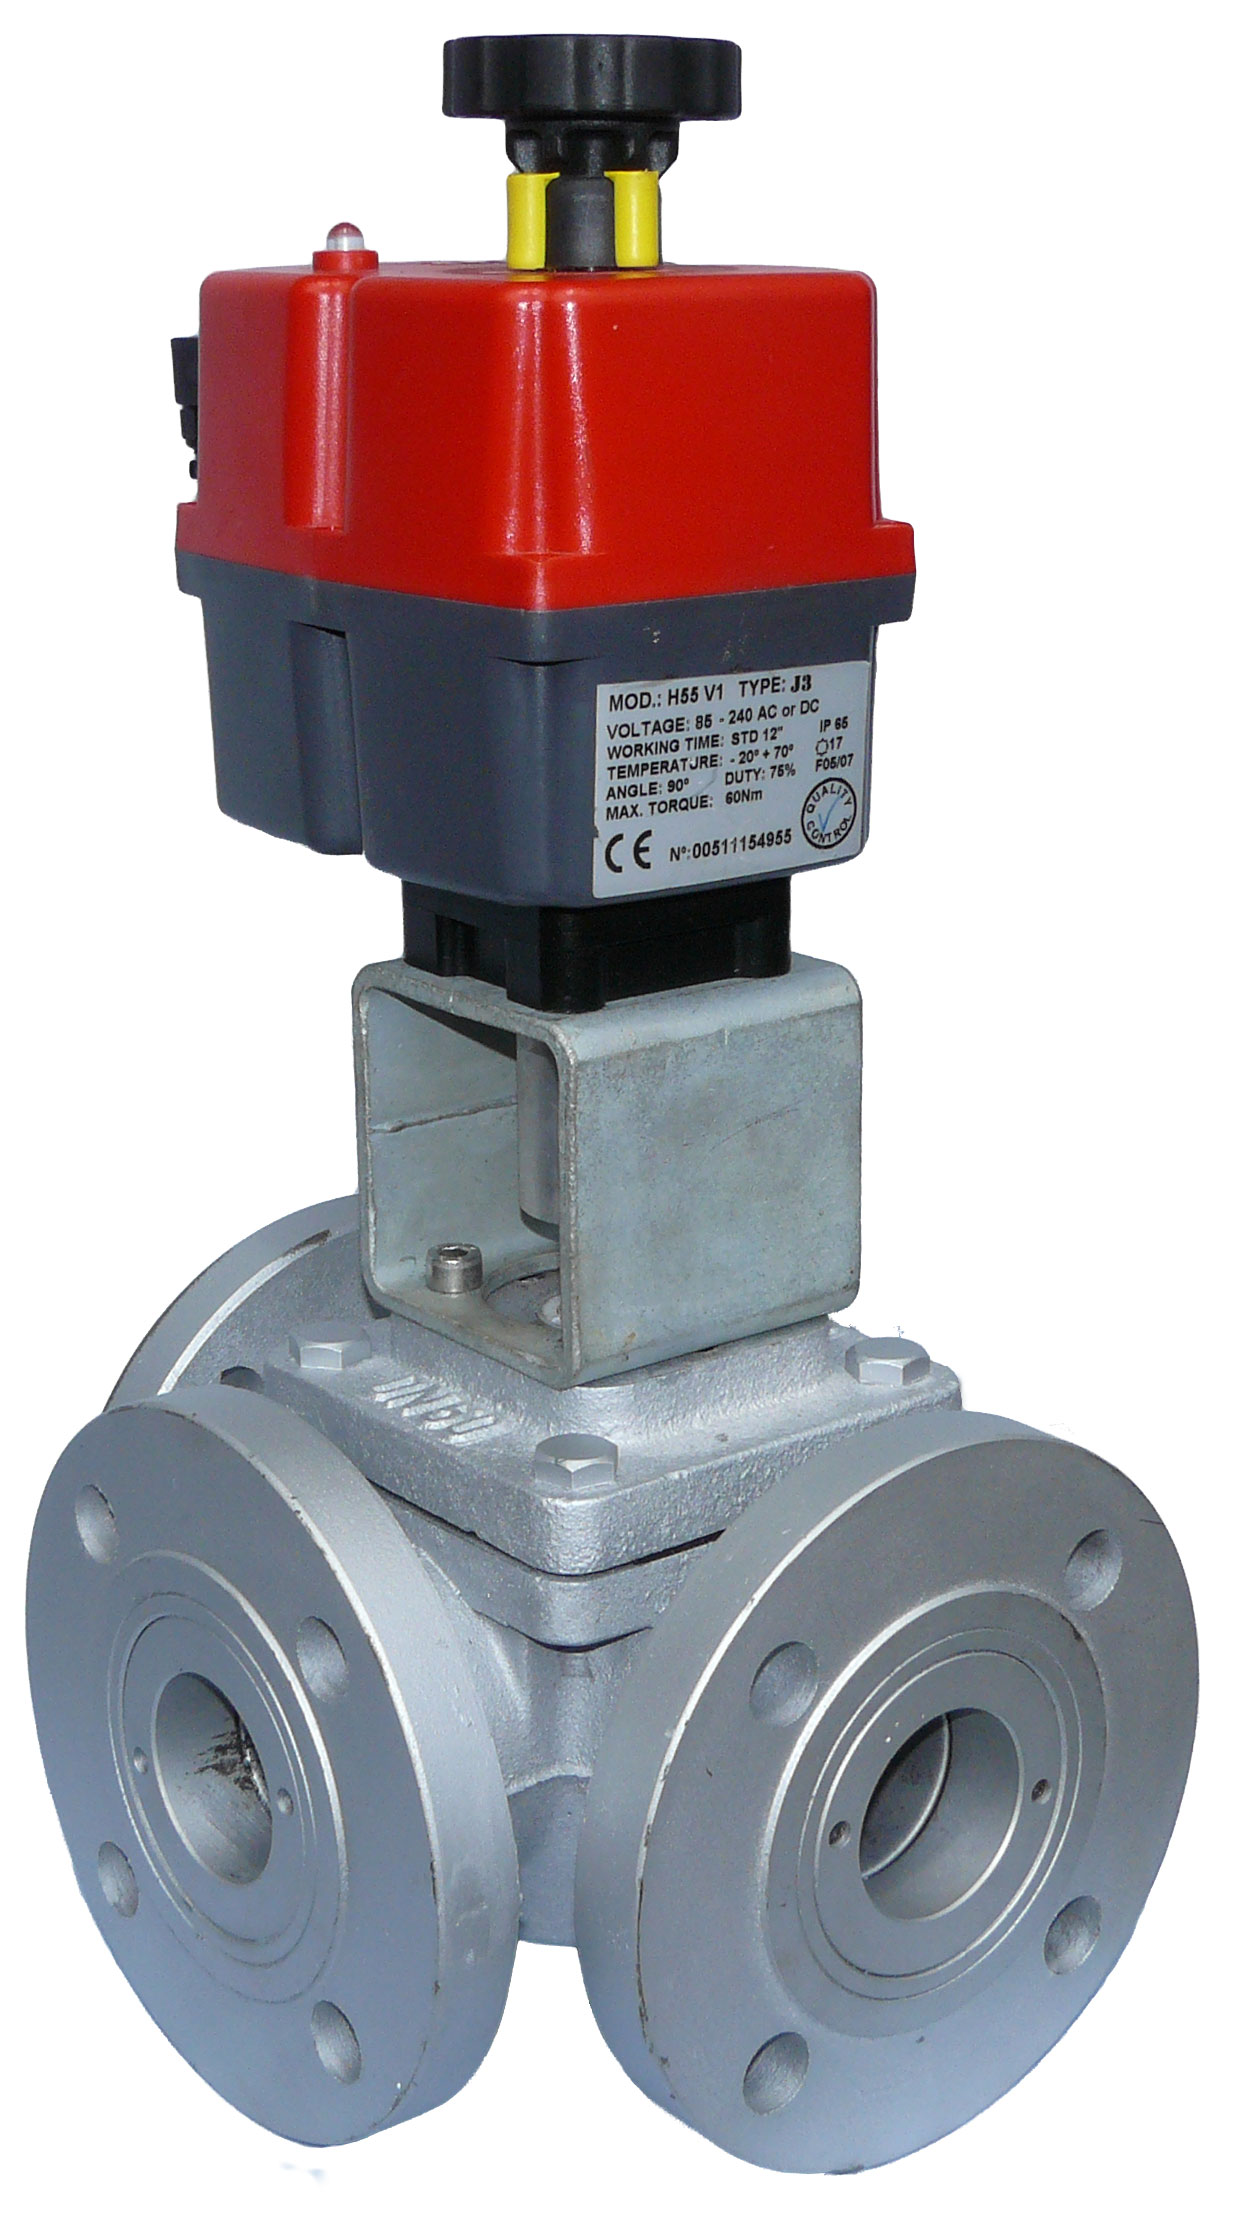
\includegraphics[scale=.09]{images/van-dien-3-nga.jpg} 
		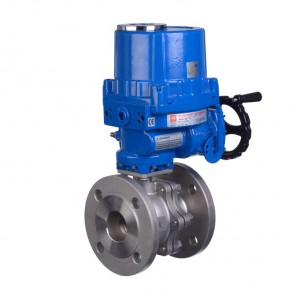
\includegraphics[scale=.65]{images/van-dien-minh-hoa.jpg} 
	\end{center}
\end{frame}

\begin{frame}{Phần van cơ thông thường}
\begin{itemize}
\justifying
	\item Phần được kết nối trực tiếp với đường ống.
	\item Tạo trạng thái đóng mở van.
	\item Gồm một số loại: van bi, van bướm, van cửa, van cầu,\ldots
\end{itemize}
\end{frame}
\begin{frame}{Phần van cơ thông thường}
\vspace{-.5cm}
\begin{center}
	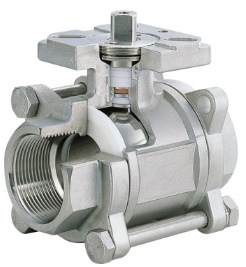
\includegraphics[scale=.7]{images/phan-co-van-bi.png} 
\end{center}
\end{frame}
\begin{frame}{Phần điều khiển bằng điện}
	\begin{itemize}
		\item Là phần quan trọng nhất của van điện.
		\item Gồm động cơ được điều khiển bởi tín hiệu điện.
		
		\item Nhận tín hiệu điều khiển làm cho động cơ quay, thay đổi trạng thái của van.
	\end{itemize}
\end{frame}

\begin{frame}{Phần điều khiển bằng điện}
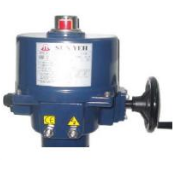
\includegraphics[scale=.7]{images/phan-dieu-khien-bang-dien.png} 
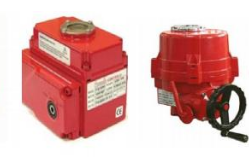
\includegraphics[scale=.7]{images/phan-dieu-khien-bang-dien-2.png} 
\end{frame}

\begin{frame}{Phần điều khiển bằng điện}
\vspace{-.5cm}
\begin{center}
	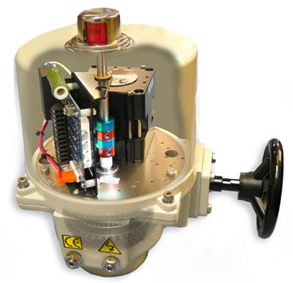
\includegraphics[scale=.65]{images/van-dien-phan-dieu-khien.png} 
\end{center}
\end{frame}
\subsection*{Nguyên lý hoạt động}
\begin{frame}{Nguyên lý hoạt động}
\justifying
Bộ điều khiển $\longrightarrow$ Động cơ trong van $\longrightarrow$ Trục van $\longrightarrow$ Tạo ra các trạng thái của van.
\end{frame}

\section{Phân loại van điện}
\begin{frame}{Phân loại van điện}
\alert{Dựa vào cấu tạo, chức năng và kiểu lắp đặt:}
\begin{itemize}
\justifying
	\item Van ĐK điện ON -- OFF.
	\item Van ĐK điện theo góc mở van.
	\item Van bướm ĐK bằng điện.
	\item Van bi ĐK bằng điện.
	\item Van điện từ.
\end{itemize}
\end{frame}

\subsection*{Van điều khiển điện ON -- OFF}
\begin{frame}{Van ĐK điện kiểu ON -- OFF}
\begin{itemize}
\justifying
\item Đóng hoặc mở hoàn toàn.
\item Không có khả năng điều tiết lưu lượng.
\item Tên gọi khác: van thường đóng hoặc van thường mở.
\item Là loại van thông dụng hiện nay.
\end{itemize}
\end{frame}
\subsection*{Van điều khiển điện theo góc mở van}
\begin{frame}{Van điều khiển điện theo góc mở van}
\begin{itemize}
\justifying
	\item Có khả năng điều tiết lưu lượng.
	\item Dùng trong các ứng dụng yêu cầu kỹ thuật cao.
\end{itemize}
\end{frame}

\subsection*{Một số loại van điện khác}
\begin{frame}{Một số loại van điện khác}
\begin{itemize}
\justifying
	\item \alert{Van bướm điều khiển bằng điện:} dùng cho các đường ống lớn.
	\item \alert{Van bi điều khiển bằng điện:} dùng cho các đường ống có kích thước nhỏ.
	\item \alert{Van điện từ:} các ứng dụng cần thời gian đáp ứng nhanh.	
\end{itemize}
\end{frame}

\section{Van bi điều khiển bằng điện}
\subsection*{Giới thiệu}
\begin{frame}{Van bi điều khiển bằng điện}
\begin{center}
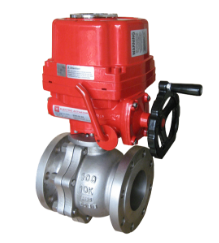
\includegraphics[scale=.75]{images/van-bi.png} 
\end{center}
\end{frame}
\begin{frame}{Các tên gọi khác}
\begin{itemize}
\justifying
	\item Van bi điện.
	\item Van bi inox điều khiển bằng điện.
	\item Van bi tự động.
	\item Van bi 2 cửa tự động.
	\item Van điện kiểu bi.
\end{itemize}
\end{frame}
\subsection*{Phân loại}
\begin{frame}{Phân loại}
	\begin{itemize}
	\justifying
		\item Điều khiển điện ON -- OFF.
		
		\item Điều khiển điện theo góc mở.
	\end{itemize}
\end{frame}

\subsection*{Cấu tạo}
\begin{frame}{Cấu tạo}
	\begin{itemize}
	\justifying
		\item Phần van cơ -- van bi: van bi inox, van bi nhựa, van bi đồng.
		
		\item Phần điều khiển điện: nhận tín hiệu điều khiển trạng thái van ở phần van cơ.
	\end{itemize}
\end{frame}

\begin{frame}{Phần van cơ của van bi}
\vspace{-.5cm}
\begin{center}
	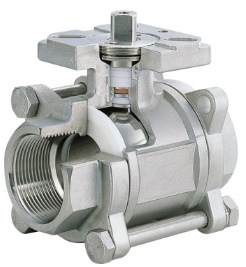
\includegraphics[scale=.7]{images/phan-co-van-bi.png} 
\end{center}
\end{frame}

\begin{frame}{Phần ĐK điện của van bi}
\vspace{-.5cm}
\begin{center}
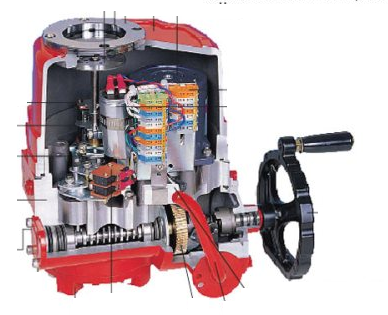
\includegraphics[scale=.6]{images/phan-dien-van-bi.png} 
\end{center}
\end{frame}

\subsection*{Nguyên lý hoạt động của van bi}
\begin{frame}{Van bi điều khiển điện ON - OFF}
\begin{itemize}
\justifying
	\item Cài đặt trạng thái của van: NO hoặc NC.
	\item Động cơ quay làm quay trục van (góc $90^0$) thay đổi trạng thái NC hoặc NO.
\end{itemize}
\end{frame}

\subsection*{Ưu và nhược điểm}
\begin{frame}{Ưu điểm}
\begin{itemize}
\justifying
	\item Kiểu lắp: lắp ren, rắc co.
	\item Không ảnh hưởng lưu lượng.
	\item Dễ thay thế sửa chữa.
	\item Hoạt động với nhiều cáp điện áp.
	\item Van bi inox chịu được nhiệt cao.
	\item Chịu áp lực lớn, cấu tạo bền, tuổi thọ tăng cao.
\end{itemize}
\end{frame}

\begin{frame}{Nhược điểm}
\begin{itemize}
\justifying
	\item Thời gian đóng mở lâu.
	\item Trọng lượng nặng, giá thành hơi cao.
\end{itemize}
\end{frame}
%--------------------------------------------------------------------------------
%--------------------------------------------------------------------------------
% Tai lieu tham khao
\section*{Tài liệu tham khảo}
\begin{frame}{Tài liệu tham khảo}
\justifying
[1]. Hoàng Minh Sơn, \textit{Thiết kế hệ thống Điều khiển quá trình}, NXB Bách Khoa Hà Nội, Năm 2009.

[2]. \href{http://vankhinen.vn/van-dieu-khien-dien-d12.html}{Van điều khiển bằng điện.}

[3]. \href{http://vankhinen.vn/van-bi-dieu-khien-dien-id49.html}{Van bi điều khiển điện.}
\end{frame}
%--------------------------------------------------------------------------------
%--------------------------------------------------------------------------------
% Tai lieu tham khao
\section*{Lời cảm ơn}
\begin{frame}
\justifying
\Large \alert{Cảm ơn Thầy và các bạn đã theo dõi phần trình bày của nhóm!}
\end{frame}
\end{document}